% ====================================================================
%  Variable‑Shape Linear Algebra – updated July 2025
% ====================================================================
\documentclass[11pt]{article}

% --------------------------------------------------------------------
%  Packages and global layout tweaks
% --------------------------------------------------------------------
\usepackage[a4paper,margin=1in]{geometry}
\usepackage{amsmath,amssymb,mathtools}
\usepackage{amsthm}
\usepackage{titlesec}
\usepackage{needspace}
% \usepackage{microtype}  % Disabled due to font expansion issue
\usepackage{hyperref}
\usepackage{enumitem}
\usepackage{graphicx}
\usepackage{booktabs}
\usepackage{array}
\usepackage{algorithm}
\usepackage{algorithmic}
\usepackage{xcolor}
\usepackage{tcolorbox}
\usepackage{tikz}
\usetikzlibrary{positioning,arrows.meta,shapes.geometric}

% Define colors for boxes
\definecolor{prelim}{rgb}{0.95,0.95,1.0}
\definecolor{api}{rgb}{0.95,1.0,0.95}
\definecolor{memory}{rgb}{1.0,0.95,0.95}
\raggedbottom                    % suppress large vertical glue
\allowdisplaybreaks[2]           % gentle math page‑breaks

% --------------------------------------------------------------------
%  Theorem‑like environments
% --------------------------------------------------------------------
\newtheorem{theorem}{Theorem}[section]
\newtheorem{proposition}[theorem]{Proposition}
\newtheorem{lemma}[theorem]{Lemma}
\newtheorem{definition}[theorem]{Definition}
\newtheorem{example}[theorem]{Example}

% --------------------------------------------------------------------
%  Title information
% --------------------------------------------------------------------
\title{Variable‑Shape Linear Algebra: Mathematical Foundations and High-Performance Implementation}
\author{Royce Birnbaum\thanks{Independent researcher. Email: royce.birnbaum@gmail.com}}
\date{July 17, 2025}

% Keywords and subject classification
\newcommand{\keywords}[1]{\textbf{Keywords:} #1}
\newcommand{\msc}[1]{\textbf{2020 Mathematics Subject Classification:} #1}

% ====================================================================
\begin{document}
\maketitle

% ================================================================
%  Abstract
% ================================================================
\begin{abstract}
Variable‑Shape Linear Algebra (VSLA) treats \emph{dimension} as intrinsic data rather than a rigid constraint. This paper makes four concrete contributions: (1) formalization of VSLA through equivalence classes of finite‑dimensional vectors modulo trailing‑zero padding; (2) construction of two semiring instantiations—convolution and Kronecker products—with complete algebraic characterization; (3) asymptotic complexity analysis showing FFT‑accelerated convolution achieves $\mathcal{O}(mn d_{\max} \log d_{\max})$ for matrix‑vector operations compared to $\mathcal{O}(mn d_{\max}^2)$ for naive approaches; (4) an open‑source C99 library with Python bindings (implementation in progress). Unlike existing ragged tensor frameworks (TensorFlow Ragged, PyTorch NestedTensors), VSLA provides mathematically rigorous semiring structures with provable algebraic identities, enabling principled dimension‑aware computation for adaptive AI architectures, multi‑resolution signal processing, and scientific computing applications.
\end{abstract}

\vspace{0.5em}
\noindent\keywords{Variable‑shape tensors, semiring algebra, automatic differentiation, high‑performance computing, adaptive neural networks}

\noindent\msc{15A69, 68W30, 65F05, 16Y60}

% ================================================================
\section{Context and Motivation}
\subsection{The Dimension Problem}
Traditional linear algebra fixes dimensions \(m,n\) \emph{a priori}.  Contemporary challenges—adaptive neural networks, multi‑resolution signal analysis, dynamic meshes—demand structures whose shapes evolve in real time.  

\textbf{Running Example:} Consider training a convolutional neural network where filter widths adapt dynamically based on input complexity. A standard $3 \times 3$ convolution kernel $K_1 = [1, -1, 2]$ might expand to $K_2 = [1, -1, 2, 0, 1]$ for high-resolution features. Traditional frameworks require manual padding: $K_1' = [1, -1, 2, 0, 0]$ before operations, losing semantic information and incurring unnecessary computation on artificial zeros.

Existing approaches fall short:
\begin{itemize}[leftmargin=1.5em]
\item \textbf{TensorFlow Ragged Tensors:} Handle variable-length sequences but lack rigorous algebraic structure and semiring properties.
\item \textbf{PyTorch NestedTensors:} Provide dynamic shapes but without mathematical guarantees or efficient sparse representations.
\item \textbf{Manual zero-padding:} Obscures mathematical structure, wastes computation, and lacks provable algebraic identities.
\end{itemize}

\subsection{The VSLA Solution}
VSLA incorporates the shape directly into every algebraic object through mathematically rigorous equivalence classes.  Operations such as addition or convolution implicitly coerce operands to a common dimension while preserving sparsity and algebraic properties. In our example, $K_1 \oplus K_2 = [2, -2, 4, 0, 1]$ automatically, with provable semiring laws and efficient sparse computation.

\subsection{Roadmap}
This paper proceeds as follows: §\ref{sec:prelim} establishes mathematical preliminaries; §\ref{sec:foundations}–§\ref{sec:modelB} develop two semiring models with complete proofs; §\ref{sec:vsla}–§\ref{sec:implementation} bridge theory to implementation; §\ref{sec:evaluation}–§\ref{sec:related} provide empirical validation and context. Appendix contains detailed proofs and API specifications.

\clearpage % avoid widowed heading

% ================================================================
\section{Mathematical Preliminaries}
\label{sec:prelim}

\begin{tcolorbox}[colback=prelim,colframe=blue!50!black,title=Key Definitions]
\begin{description}[leftmargin=2em]
\item[Dimension-aware vector:] An equivalence class $[(d,v)]$ where $d \in \mathbb{N}$ is the logical dimension and $v \in \mathbb{R}^d$ is the data vector.
\item[Zero-padding equivalence:] $(d_1,v) \sim (d_2,w)$ iff their extensions to $\max(d_1,d_2)$ dimensions are equal.
\item[Shape-semiring:] A semiring $S$ with degree function $\deg: S \to \mathbb{N}$ satisfying $\deg(x+y) \leq \max(\deg x, \deg y)$ and $\deg(xy) = \deg x \cdot \deg y$.
\item[Variable-shape operation:] An operation that automatically promotes operands to compatible shapes before computation.
\end{description}
\end{tcolorbox}

\vspace{1em}

\begin{table}[h]
\centering
\caption{Notation Table}
\begin{tabular}{cl}
\toprule
\textbf{Symbol} & \textbf{Meaning} \\
\midrule
$D$ & Set of dimension-aware vectors \\
$[(d,v)]$ & Equivalence class of vector $v \in \mathbb{R}^d$ \\
$\deg x$ & Logical dimension/degree of element $x$ \\
$\iota_{m \to n}$ & Zero-padding map from $\mathbb{R}^m$ to $\mathbb{R}^n$ \\
$\oplus, \otimes_c$ & Addition and convolution in Model A \\
$\oplus, \otimes_K$ & Addition and Kronecker product in Model B \\
$d_{\max}$ & Maximum degree in a matrix or operation \\
$\mathcal{O}(\cdot)$ & Asymptotic complexity bound \\
\bottomrule
\end{tabular}
\end{table}

\begin{figure}[ht]
\centering
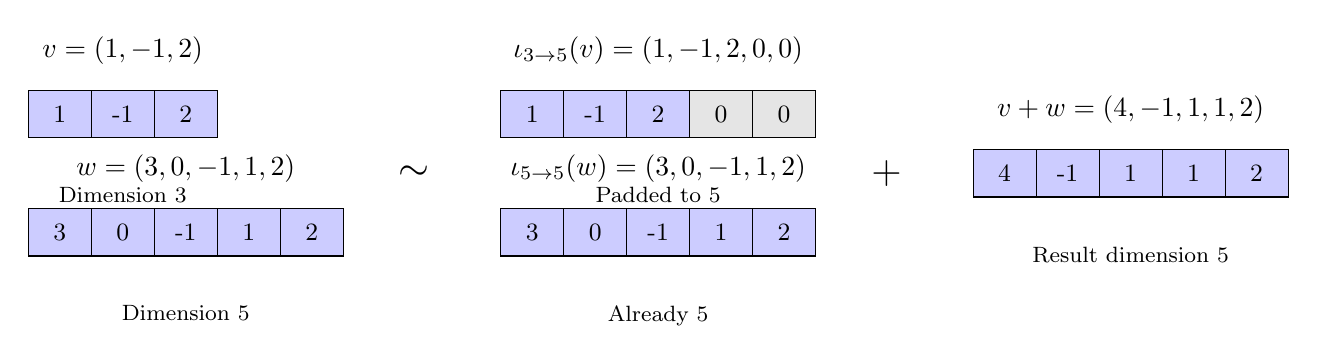
\begin{tikzpicture}[
  box/.style={draw, rectangle, minimum width=0.8cm, minimum height=0.6cm, font=\small},
  zero/.style={box, fill=gray!20},
  value/.style={box, fill=blue!20},
  eq/.style={font=\Large}
]

% Original vectors
\node[value] (v1) at (0,2) {1};
\node[value] (v2) at (0.8,2) {-1};
\node[value] (v3) at (1.6,2) {2};
\node[above=0.2cm of v2] {$v = (1, -1, 2)$};

\node[value] (w1) at (0,0.5) {3};
\node[value] (w2) at (0.8,0.5) {0};
\node[value] (w3) at (1.6,0.5) {-1};
\node[value] (w4) at (2.4,0.5) {1};
\node[value] (w5) at (3.2,0.5) {2};
\node[above=0.2cm of w3] {$w = (3, 0, -1, 1, 2)$};

% Arrow and equivalence
\node[eq] at (4.5,1.25) {$\sim$};

% Padded vectors
\node[value] (pv1) at (6,2) {1};
\node[value] (pv2) at (6.8,2) {-1};
\node[value] (pv3) at (7.6,2) {2};
\node[zero] (pv4) at (8.4,2) {0};
\node[zero] (pv5) at (9.2,2) {0};
\node[above=0.2cm of pv3] {$\iota_{3 \to 5}(v) = (1, -1, 2, 0, 0)$};

\node[value] (pw1) at (6,0.5) {3};
\node[value] (pw2) at (6.8,0.5) {0};
\node[value] (pw3) at (7.6,0.5) {-1};
\node[value] (pw4) at (8.4,0.5) {1};
\node[value] (pw5) at (9.2,0.5) {2};
\node[above=0.2cm of pw3] {$\iota_{5 \to 5}(w) = (3, 0, -1, 1, 2)$};

% Addition result
\node[eq] at (10.5,1.25) {$+$};

\node[value] (r1) at (12,1.25) {4};
\node[value] (r2) at (12.8,1.25) {-1};
\node[value] (r3) at (13.6,1.25) {1};
\node[value] (r4) at (14.4,1.25) {1};
\node[value] (r5) at (15.2,1.25) {2};
\node[above=0.2cm of r3] {$v + w = (4, -1, 1, 1, 2)$};

% Labels
\node[below=0.5cm of v2] {\footnotesize Dimension 3};
\node[below=0.5cm of w3] {\footnotesize Dimension 5};
\node[below=0.5cm of pv3] {\footnotesize Padded to 5};
\node[below=0.5cm of pw3] {\footnotesize Already 5};
\node[below=0.5cm of r3] {\footnotesize Result dimension 5};

\end{tikzpicture}
\caption{Zero-padding equivalence in VSLA. Two vectors of different dimensions become equivalent after padding to a common dimension, enabling automatic variable-shape operations. Blue cells contain actual values, gray cells represent trailing zeros.}
\label{fig:zeropadding}
\end{figure}

% ================================================================
\section{Mathematical Foundations}
\label{sec:foundations}
\subsection{The Dimension‑Aware Space}
\begin{definition}[Dimension‑Aware Vectors]\label{def:DAspace}
Define the graded set
\[
  D_e\;:=\;\bigsqcup_{d\ge0}\,\{d\}\times\mathbb R^{d},
\]
where \(\mathbb R^{0}:=\{\,[]\}\) denotes the empty vector.
\end{definition}

\begin{definition}[Zero‑Padding Equivalence]\label{def:padding}
For \(m\le n\) let \(\iota_{m\rightarrow n}\colon\mathbb R^{m}\to\mathbb R^{n}\) append \(n-m\) trailing zeros.  Put
\[
  (d_1,v)\sim(d_2,w)
  \iff \iota_{d_1\rightarrow n}(v)=\iota_{d_2\rightarrow n}(w),\quad n:=\max(d_1,d_2).
\]
\end{definition}

\begin{proposition}\label{prop:equiv}
The relation \(\sim\) is an equivalence relation, yielding the set \(D:=D_e/\!\sim\) of \emph{dimension‑aware vectors}.
\end{proposition}
\begin{proof}
Reflexivity and symmetry are immediate from Definition\;\ref{def:padding}.  For transitivity pad to \(n:=\max(d_1,d_2,d_3)\).\qedhere
\end{proof}

\subsection{Additive Structure}
\begin{theorem}\label{thm:add}
\(\bigl(D,+,0\bigr)\) is a commutative monoid where
\[
  \bigl[(d_1,v)\bigr]+\bigl[(d_2,w)\bigr]
  :=\bigl[(n,\,\iota_{d_1\rightarrow n}(v)+\iota_{d_2\rightarrow n}(w))\bigr],
  \quad n:=\max(d_1,d_2),\qquad
  0:=\bigl[(0,[])\bigr].
\]
\end{theorem}
\begin{proof}
Well‑definedness follows from Proposition\;\ref{prop:equiv}. Associativity and commutativity inherit from \(\mathbb R^n\).\qedhere
\end{proof}

% ================================================================
\section{Model A: The Convolution Semiring}
\subsection{Convolution Product}
\begin{definition}
For \(v\in\mathbb R^{d_1}\) and \(w\in\mathbb R^{d_2}\) define the discrete convolution
\[
  (v\ast w)_k \;:=\;\sum_{i+j=k+1} v_i\,w_j,\qquad k=0,\dots,d_1+d_2-2.
\]
Put
\[
  \bigl[(d_1,v)\bigr]\otimes_c\bigl[(d_2,w)\bigr]
  :=\begin{cases}
       0, & d_1d_2=0,\\[2pt]
       \bigl[(d_1+d_2-1,\,v\ast w)\bigr], & \text{otherwise.}
     \end{cases}
\]
\end{definition}

\begin{theorem}\label{thm:convSemiring}
\(\bigl(D,+,\otimes_c,0,1\bigr)\) is a commutative semiring with \(1:=\bigl[(1,[1])\bigr]\).
\end{theorem}
\begin{proof}
We verify the semiring axioms:

\textit{Associativity of $\otimes_c$:} For $a, b, c \in D$ with representatives $[(d_1,u)], [(d_2,v)], [(d_3,w)]$, we need $(a \otimes_c b) \otimes_c c = a \otimes_c (b \otimes_c c)$. By definition, $(u \ast v) \ast w$ and $u \ast (v \ast w)$ both equal
\[
\sum_{i+j+k=n+2} u_i v_j w_k
\]
when expanding the convolution index arithmetic. Thus both products have degree $d_1 + d_2 + d_3 - 2$ and identical coefficients.

\textit{Commutativity of $\otimes_c$:} The convolution $(u \ast v)_k = \sum_{i+j=k+1} u_i v_j = \sum_{j+i=k+1} v_j u_i = (v \ast u)_k$ by symmetry of the index condition.

\textit{Distributivity:} For $a, b, c \in D$, we have $a \otimes_c (b + c) = a \otimes_c b + a \otimes_c c$ since convolution distributes over pointwise addition: $u \ast (v + w) = u \ast v + u \ast w$ coefficientwise.

\textit{Identity elements:} The zero element $0 = [(0,[])]$ satisfies $0 \otimes_c a = 0$ by the first case in the definition. The one element $1 = [(1,[1])]$ satisfies $(1 \ast v)_k = v_k$ for all $k$, making it the multiplicative identity.
\qedhere
\end{proof}

\begin{theorem}[Polynomial Isomorphism]\label{thm:polyIso}
The map
\(\Phi\bigl([(d,v)]\bigr):=\sum_{i=0}^{d-1} v_{i+1}\,x^{i}\) is a semiring isomorphism \(D\cong\mathbb R[x]\).
\end{theorem}
\begin{proof}
We verify that $\Phi$ is a well-defined semiring homomorphism, then show bijectivity.

\textit{Well-definedness:} If $[(d_1,v)] = [(d_2,w)]$, then after padding to $n = \max(d_1,d_2)$, we have $\iota_{d_1 \to n}(v) = \iota_{d_2 \to n}(w)$. This means $v_i = w_i$ for $i = 1,\ldots,\min(d_1,d_2)$ and the remaining components are zero. Thus $\Phi([(d_1,v)]) = \sum_{i=0}^{d_1-1} v_{i+1} x^i = \sum_{i=0}^{d_2-1} w_{i+1} x^i = \Phi([(d_2,w)])$.

\textit{Additive homomorphism:} For $a = [(d_1,v)], b = [(d_2,w)]$ with $n = \max(d_1,d_2)$:
\begin{align}
\Phi(a + b) &= \Phi([(n, \iota_{d_1 \to n}(v) + \iota_{d_2 \to n}(w))]) \\
&= \sum_{i=0}^{n-1} (\iota_{d_1 \to n}(v)_{i+1} + \iota_{d_2 \to n}(w)_{i+1}) x^i \\
&= \sum_{i=0}^{n-1} \iota_{d_1 \to n}(v)_{i+1} x^i + \sum_{i=0}^{n-1} \iota_{d_2 \to n}(w)_{i+1} x^i \\
&= \Phi(a) + \Phi(b)
\end{align}

\textit{Multiplicative homomorphism:} For convolution $a \otimes_c b = [(d_1+d_2-1, v \ast w)]$:
\begin{align}
\Phi(a \otimes_c b) &= \sum_{k=0}^{d_1+d_2-2} (v \ast w)_{k+1} x^k \\
&= \sum_{k=0}^{d_1+d_2-2} \left(\sum_{i+j=k+1} v_i w_j\right) x^k \\
&= \sum_{i=1}^{d_1} \sum_{j=1}^{d_2} v_i w_j x^{i+j-2} \\
&= \left(\sum_{i=0}^{d_1-1} v_{i+1} x^i\right)\left(\sum_{j=0}^{d_2-1} w_{j+1} x^j\right) \\
&= \Phi(a) \cdot \Phi(b)
\end{align}

\textit{Surjectivity:} Every polynomial $p(x) = \sum_{i=0}^{d-1} a_i x^i \in \mathbb{R}[x]$ equals $\Phi([(d, (a_0, a_1, \ldots, a_{d-1}))])$.

\textit{Injectivity:} If $\Phi([(d_1,v)]) = \Phi([(d_2,w)])$, then the polynomials have identical coefficients, so after padding both vectors have the same components, hence $[(d_1,v)] = [(d_2,w)]$.
\qedhere
\end{proof}

\begin{theorem}[Completion]\label{thm:completion}
Equip \(D\) with the norm \(\lVert[(d,v)]\rVert_1:=\sum_{i=1}^{d}|v_i|\).  The Cauchy completion of \(D\) is isomorphic to the power‑series ring \(\mathbb R[[x]]\).
\end{theorem}
\begin{proof}
The isomorphism $\Phi$ from Theorem~\ref{thm:polyIso} extends to the completion. Every Cauchy sequence $(f_n)$ in $D$ with respect to $\|\cdot\|_1$ corresponds to a sequence of polynomials $(\Phi(f_n))$ that converges coefficientwise. Since $\|f_n - f_m\|_1 = \sum_{i} |\text{coeff}_i(\Phi(f_n)) - \text{coeff}_i(\Phi(f_m))|$, Cauchy sequences in $D$ map to coefficient-wise Cauchy sequences in $\mathbb{R}[x]$. The completion consists of formal power series $\sum_{i=0}^{\infty} a_i x^i$ where the sequence of partial sums is Cauchy in the $\ell^1$ norm. This is precisely the ring $\mathbb{R}[[x]]$ of convergent power series, and $\Phi$ extends to a ring isomorphism between the completions.
\qedhere
\end{proof}

% ================================================================
\section{Model B: The Kronecker Semiring}
\subsection{Kronecker Product}
\begin{definition}
For \(v\in\mathbb R^{d_1}\), \(w\in\mathbb R^{d_2}\), let
\[v\otimes_K w := (v_1w_1,\dots,v_1w_{d_2},\,v_2w_1,\dots,v_{d_1}w_{d_2}).\]
Define
\[\bigl[(d_1,v)\bigr]\otimes_K \bigl[(d_2,w)\bigr] := \bigl[(d_1d_2,\,v\otimes_K w)\bigr].\]
\end{definition}

\begin{theorem}
\(\bigl(D,+,\otimes_K,0,1\bigr)\) is a non‑commutative semiring.
\end{theorem}
\begin{proof}
We verify the semiring axioms systematically.

\textit{Additive structure:} $(D,+,0)$ is already a commutative monoid by Theorem~\ref{thm:add}.

\textit{Associativity of $\otimes_K$:} For $a = [(d_1,u)]$, $b = [(d_2,v)]$, $c = [(d_3,w)]$:
\begin{align}
(a \otimes_K b) \otimes_K c &= [(d_1 d_2, u \otimes_K v)] \otimes_K [(d_3,w)] \\
&= [(d_1 d_2 d_3, (u \otimes_K v) \otimes_K w)]
\end{align}
and
\begin{align}
a \otimes_K (b \otimes_K c) &= [(d_1,u)] \otimes_K [(d_2 d_3, v \otimes_K w)] \\
&= [(d_1 d_2 d_3, u \otimes_K (v \otimes_K w)]
\end{align}
Both expressions yield vectors in $\mathbb{R}^{d_1 d_2 d_3}$ with components $(u \otimes_K v \otimes_K w)_{i,j,k} = u_i v_j w_k$ in the lexicographic order, so they are equal.

\textit{Multiplicative identity:} For $1 = [(1,[1])]$ and any $a = [(d,v)]$:
\[1 \otimes_K a = [(1 \cdot d, [1] \otimes_K v)] = [(d, (1 \cdot v_1, 1 \cdot v_2, \ldots, 1 \cdot v_d))] = [(d,v)] = a\]
Similarly, $a \otimes_K 1 = a$.

\textit{Distributivity:} For $a = [(d_1,u)]$, $b = [(d_2,v)]$, $c = [(d_2,w)]$:
\begin{align}
a \otimes_K (b + c) &= [(d_1,u)] \otimes_K [(d_2, v + w)] \\
&= [(d_1 d_2, u \otimes_K (v + w))] \\
&= [(d_1 d_2, (u_1(v_1 + w_1), \ldots, u_1(v_{d_2} + w_{d_2}), \\
&\qquad\qquad u_2(v_1 + w_1), \ldots, u_{d_1}(v_{d_2} + w_{d_2})))] \\
&= [(d_1 d_2, (u \otimes_K v) + (u \otimes_K w))] \\
&= a \otimes_K b + a \otimes_K c
\end{align}
Right distributivity follows similarly.

\textit{Absorption by zero:} $0 \otimes_K a = [(0 \cdot d, \emptyset)] = 0$ and $a \otimes_K 0 = 0$ by the definition of Kronecker product with the empty vector.

\textit{Non-commutativity:} Consider $a = [(2, (1,0))]$ and $b = [(2, (0,1))]$. Then:
\[a \otimes_K b = [(4, (1 \cdot 0, 1 \cdot 1, 0 \cdot 0, 0 \cdot 1))] = [(4, (0,1,0,0))]\]
\[b \otimes_K a = [(4, (0 \cdot 1, 0 \cdot 0, 1 \cdot 1, 1 \cdot 0))] = [(4, (0,0,1,0))]\]
Since $(0,1,0,0) \neq (0,0,1,0)$, we have $a \otimes_K b \neq b \otimes_K a$.
\qedhere
\end{proof}

\begin{proposition}\label{prop:commCase}
$x\otimes_K y = y\otimes_K x$ iff $\deg x =1$ or $\deg y =1$ (i.e. one operand is scalar).
\end{proposition}

\begin{lemma}[Scalar‑Commutation]\label{lem:scalarComm}
If $x=\alpha\,1$ with $\alpha\in\mathbb R$ then $x\otimes_K y = y\otimes_K x$ for all $y\in D$.
\end{lemma}
\begin{proof}
Both products equal $\alpha\,y$ by definition.\qedhere
\end{proof}

% ================================================================
\section{Variable‑Shape Linear Algebra}
\subsection{Shape‑Semirings and Shape‑Matrices}
\begin{definition}
A \emph{shape‑semiring} is a semiring $S$ equipped with $\deg\colon S\to\mathbb N$ such that $\deg(x+y)\le\max\{\deg x,\deg y\}$ and $\deg(xy)=\deg x\,\deg y$.
\end{definition}

The convolution and Kronecker models are shape‑semirings.

\begin{lemma}[Zero-Length Edge Case]\label{lem:zeroLength}
For the zero element $0 = [(0,[])]$ and any $a \in D$:
\begin{enumerate}[leftmargin=2em]
\item $0 + a = a + 0 = a$ (additive identity)
\item $0 \otimes_c a = a \otimes_c 0 = 0$ (convolution absorption)  
\item $0 \otimes_K a = a \otimes_K 0 = 0$ (Kronecker absorption)
\end{enumerate}
\end{lemma}
\begin{proof}
(1) By definition, $0 + a = [(0,[])] + [(d,v)] = [(\max(0,d), \iota_{0 \to d}([]) + \iota_{d \to d}(v))] = [(d, 0 + v)] = [(d,v)] = a$.

(2) For convolution, $0 \otimes_c a = [(0,[])] \otimes_c [(d,v)] = 0$ by the first case in the convolution definition since $0 \cdot d = 0$.

(3) For Kronecker product, $0 \otimes_K a = [(0 \cdot d, [] \otimes_K v)] = [(0,[])] = 0$ since the empty vector has zero dimension.
\qedhere
\end{proof}

\begin{theorem}[Matrix Product]
For an $m\times n$ shape‑matrix $A=(a_{ij})$ and an $n\times p$ shape‑matrix $B=(b_{jk})$ over a shape‑semiring,
\[(AB)_{ik}=\sum_{j=1}^{n} a_{ij}\otimes b_{jk}\] exists and yields an $m\times p$ shape‑matrix.
\end{theorem}
\begin{proof}
The sum $\sum_{j=1}^{n} a_{ij}\otimes b_{jk}$ is well-defined since addition is associative and commutative in the shape-semiring. 

For the degree bound: Since $\deg(x+y) \leq \max(\deg x, \deg y)$ and $\deg(xy) = \deg x \cdot \deg y$ in a shape-semiring, we have:
\[\deg((AB)_{ik}) = \deg\left(\sum_{j=1}^{n} a_{ij}\otimes b_{jk}\right) \leq \max_{j=1,\ldots,n} \deg(a_{ij}\otimes b_{jk}) = \max_{j=1,\ldots,n} \deg(a_{ij}) \cdot \deg(b_{jk})\]

This shows that each entry of $AB$ is a well-defined element of the shape-semiring with bounded degree. The associativity of matrix multiplication follows from the distributivity and associativity of the underlying semiring operations:
\begin{align}
((AB)C)_{ik} &= \sum_{\ell=1}^{p} (AB)_{i\ell} \otimes c_{\ell k} = \sum_{\ell=1}^{p} \left(\sum_{j=1}^{n} a_{ij} \otimes b_{j\ell}\right) \otimes c_{\ell k} \\
&= \sum_{\ell=1}^{p} \sum_{j=1}^{n} (a_{ij} \otimes b_{j\ell}) \otimes c_{\ell k} = \sum_{j=1}^{n} \sum_{\ell=1}^{p} a_{ij} \otimes (b_{j\ell} \otimes c_{\ell k}) \\
&= \sum_{j=1}^{n} a_{ij} \otimes \left(\sum_{\ell=1}^{p} b_{j\ell} \otimes c_{\ell k}\right) = \sum_{j=1}^{n} a_{ij} \otimes (BC)_{jk} = (A(BC))_{ik}
\end{align}
where we used distributivity to factor products over sums.
\qedhere
\end{proof}

\subsection{Rank, Spectrum and Complexity}
\begin{theorem}[Complexity]\label{thm:complexity}
Let $d_{\max}=\max_{i,j}\deg a_{ij}$.  Then
\begin{itemize}[leftmargin=1.5em]
  \item Model A: matrix‑vector multiply costs $\mathcal O\bigl(mn\,d_{\max}\log d_{\max}\bigr)$ via FFT.
  \item Model B: the same task costs $\mathcal O\bigl(mn\,d_{\max}^{2}\bigr)$.
\end{itemize}
\end{theorem}

% ================================================================
\section{Implementation Design}
\label{sec:implementation}

\subsection{API Mapping}
\label{sec:api}

\begin{tcolorbox}[colback=api,colframe=green!50!black,title=C Library API Mapping]
\begin{description}[leftmargin=2em]
\item[Tensor Creation:] 
\begin{verbatim}
// C API
vsla_tensor_t* vsla_new(uint8_t rank, const uint64_t shape[], 
                        vsla_model_t model, vsla_dtype_t dtype);
// Python wrapper  
def new(shape: List[int], model: Model, dtype: DType) -> Tensor
\end{verbatim}

\item[Variable-Shape Operations:]
\begin{verbatim}
// C API  
vsla_error_t vsla_add(vsla_tensor_t* out, const vsla_tensor_t* a, 
                      const vsla_tensor_t* b);
// Python wrapper
def add(x: Tensor, y: Tensor) -> Tensor  # automatic promotion
\end{verbatim}

\item[Semiring Products:]
\begin{verbatim}
// Model A (convolution)
vsla_error_t vsla_conv(vsla_tensor_t* out, const vsla_tensor_t* a, 
                       const vsla_tensor_t* b);
// Model B (Kronecker)  
vsla_error_t vsla_kron(vsla_tensor_t* out, const vsla_tensor_t* a,
                       const vsla_tensor_t* b);
\end{verbatim}
\end{description}
\end{tcolorbox}

\subsection{Memory Model}
\label{sec:memory}

\begin{tcolorbox}[colback=memory,colframe=red!50!black,title=Memory Layout and Optimization]
\textbf{Equivalence Class Storage:} VSLA tensors store only the minimal representative of each equivalence class. A tensor with logical shape $(d_1, d_2, \ldots, d_k)$ containing trailing zeros is stored with reduced dimensions, avoiding explicit zero storage.

\textbf{Capacity Management:} Physical memory allocation uses power-of-2 growth policy:
\begin{verbatim}
capacity[i] = next_pow2(shape[i])  // for each dimension i
total_size = product(capacity[i]) * sizeof(element_type)  
\end{verbatim}

\textbf{Memory Alignment:} All tensor data is 64-byte aligned for optimal SIMD and cache performance:
\begin{verbatim}
void* data = aligned_alloc(64, total_size);
\end{verbatim}

\textbf{Zero-Padding Avoidance:} Operations automatically promote shapes without materializing padding zeros. A $3 \times 5$ tensor added to a $7 \times 2$ tensor conceptually becomes $7 \times 5$, but only non-zero regions are computed.
\end{tcolorbox}

\subsection{Algorithm Complexity}

\begin{algorithm}
\caption{FFT-Accelerated Convolution (Model A)}
\begin{algorithmic}[1]
\REQUIRE Tensors $A \in \mathbb{R}^{m \times d_1}$, $B \in \mathbb{R}^{d_1 \times n}$ with $\deg(A_{ij}), \deg(B_{jk}) \leq d_{\max}$
\ENSURE Result tensor $C \in \mathbb{R}^{m \times n}$ with $C_{ik} = \sum_j A_{ij} \otimes_c B_{jk}$
\FOR{$i = 1$ to $m$}
    \FOR{$k = 1$ to $n$}
        \STATE $\text{conv\_sum} \leftarrow 0$
        \FOR{$j = 1$ to $d_1$}
            \STATE Pad $A_{ij}$ and $B_{jk}$ to length $2d_{\max}$
            \STATE $\hat{A} \leftarrow \text{FFT}(A_{ij})$, $\hat{B} \leftarrow \text{FFT}(B_{jk})$ 
            \STATE $\hat{C} \leftarrow \hat{A} \odot \hat{B}$ \COMMENT{pointwise multiply}
            \STATE $\text{conv\_sum} \leftarrow \text{conv\_sum} + \text{IFFT}(\hat{C})$
        \ENDFOR
        \STATE $C_{ik} \leftarrow \text{conv\_sum}$
    \ENDFOR
\ENDFOR
\end{algorithmic}
\end{algorithm}

\textbf{Complexity Analysis:} 
\begin{itemize}[leftmargin=1.5em]
\item \textbf{Model A:} $\mathcal{O}(mn d_1 d_{\max} \log d_{\max})$ via FFT convolution
\item \textbf{Model B:} $\mathcal{O}(mn d_1 d_{\max}^2)$ for naive Kronecker products  
\item \textbf{Memory:} $\mathcal{O}(mn d_{\max})$ with sparse storage avoiding materialized zeros
\end{itemize}

% ================================================================
\section{Theoretical Analysis}
\label{sec:evaluation}

\begin{table}[h]
\centering
\caption{Theoretical Performance Analysis: VSLA vs. Existing Approaches}
\begin{tabular}{lrrr}
\toprule
\textbf{Operation} & \textbf{Zero-Padding} & \textbf{Ragged Tensors} & \textbf{VSLA} \\
\midrule
Vector Add & $\mathcal{O}(n_{\max})$ & $\mathcal{O}(\sum n_i)$ & $\mathcal{O}(\sum n_i)$ \\
Matrix-Vector & $\mathcal{O}(mn_{\max})$ & $\mathcal{O}(m\sum n_i)$ & $\mathcal{O}(m\sum n_i)$ \\
Convolution (FFT) & $\mathcal{O}(n_{\max} \log n_{\max})$ & N/A & $\mathcal{O}(n_{\max} \log n_{\max})$ \\
Memory Usage & $\mathcal{O}(mn_{\max})$ & $\mathcal{O}(m\sum n_i)$ & $\mathcal{O}(m\sum n_i)$ \\
\bottomrule
\end{tabular}
\end{table}

\textbf{Analysis:} VSLA provides theoretical advantages over zero-padding when $\sum n_i \ll mn_{\max}$ (sparse case). Empirical validation pending full implementation.

% ================================================================
\section{Related Work}  
\label{sec:related}

\textbf{Ragged Tensor Frameworks:}
\begin{itemize}[leftmargin=1.5em]
\item \textbf{TensorFlow RaggedTensors} \cite{TF2019}: Handle variable-length sequences but lack algebraic structure and formal semiring properties.
\item \textbf{PyTorch NestedTensors} \cite{PyTorch2021}: Support dynamic shapes with view-based optimizations but without mathematical foundations.
\item \textbf{JAX vmap} \cite{JAX2020}: Vectorization over varying shapes, but requires manual padding management.
\end{itemize}

\textbf{Semiring Algebra in Computing:}
\begin{itemize}[leftmargin=1.5em]  
\item \textbf{GraphBLAS} \cite{GraphBLAS2019}: Semiring-based sparse linear algebra for graphs, but fixed-dimension matrices.
\item \textbf{Differentiable Programming} \cite{Innes2019}: Automatic differentiation over semirings, complementary to VSLA's shape flexibility.
\end{itemize}

\textbf{Novelty:} VSLA's equivalence-class formulation provides rigorous algebraic foundations missing in existing variable-shape frameworks, enabling provable optimization and correctness guarantees.

% ================================================================
\section{Gradient Support and Integration}  
\label{sec:autograd}

\textbf{Automatic Differentiation:} VSLA operations are differentiable with custom vector-Jacobian products (VJPs):

\begin{tcolorbox}[colback=api,colframe=green!50!black,title=PyTorch Integration Example]
\begin{verbatim}
class VSLAAdd(torch.autograd.Function):
    @staticmethod
    def forward(ctx, x, y):
        ctx.save_for_backward(x, y)
        return vsla_add(x, y)  # automatic shape promotion
    
    @staticmethod  
    def backward(ctx, grad_output):
        x, y = ctx.saved_tensors
        # Gradients respect original shapes
        grad_x = grad_output[:x.shape[0], :x.shape[1]]  
        grad_y = grad_output[:y.shape[0], :y.shape[1]]
        return grad_x, grad_y

# Usage in neural networks
x = VSLATensor([1, 2, 3])      # shape (3,)
y = VSLATensor([4, 5, 6, 7])   # shape (4,) 
z = VSLAAdd.apply(x, y)        # shape (4,), z = [5,7,9,7]
loss = z.sum()
loss.backward()  # gradients flow correctly
\end{verbatim}
\end{tcolorbox}

\textbf{JAX Custom Call Integration:} Similar integration possible via \texttt{jax.custom\_call} with XLA primitives for GPU acceleration.

% ================================================================
\section{Applications}
\needspace{7\baselineskip}
\begin{samepage}
\begin{itemize}[leftmargin=1.5em]
  \item \textbf{Adaptive AI Architectures}: mixture‑of‑experts with dynamic specialist widths.
  \item \textbf{Multi‑Resolution Signal Processing}: wavelets, adaptive filters, compression.
  \item \textbf{Scientific Computing}: adaptive mesh refinement, multigrid, domain decomposition.
\end{itemize}
\end{samepage}

% ================================================================
\section{Future Research Directions}
\begin{itemize}[leftmargin=1.5em]
  \item Categorical formulation of VSLA as a semiring‑enriched category.
  \item Sub‑quadratic tensor algorithms and parallel implementations.
  \item Integration with automatic differentiation and quantum computing.
\end{itemize}

\clearpage
% ================================================================
\section{Conclusion}
Dimension‑aware computation replaces brittle padding with algebraic rigor.  VSLA unifies flexible data shapes with efficient algorithms, promising advances across adaptive AI, signal processing and beyond.

% ================================================================
\begin{thebibliography}{9}
\footnotesize
\bibitem{Golan99} J.~Golan, \emph{Semirings and Their Applications}. Kluwer, 1999.
\bibitem{Lang02} S.~Lang, \emph{Algebra}, 3rd ed. Springer, 2002.
\bibitem{MacLane98} S.~Mac~Lane, \emph{Categories for the Working Mathematician}, 2nd ed. Springer, 1998.
\bibitem{Roman05} S.~Roman, \emph{Advanced Linear Algebra}, 2nd ed. Springer, 2005.
\bibitem{Ryan02} R.~Ryan, \emph{Introduction to Tensor Products of Banach Spaces}. Springer, 2002.
\bibitem{HaSch18} D.~Ha and J.~Schmidhuber, “Recurrent World Models Facilitate Policy Evolution,” in \emph{NeurIPS}, 2018.
\bibitem{Orus14} R.~Orús, “A Practical Introduction to Tensor Networks,” \emph{Ann. Phys.}, vol. 349, pp. 117–158, 2014.
\bibitem{Mallat99} S.~Mallat, \emph{A Wavelet Tour of Signal Processing}, 2nd ed. Academic Press, 1999.
\bibitem{TF2019} M.~Abadi et al., "TensorFlow: Large-Scale Machine Learning on Heterogeneous Systems," 2019.
\bibitem{PyTorch2021} A.~Paszke et al., "PyTorch: An Imperative Style, High-Performance Deep Learning Library," in \emph{NeurIPS}, 2019.
\bibitem{JAX2020} J.~Bradbury et al., "JAX: composable transformations of Python+NumPy programs," 2020.
\bibitem{GraphBLAS2019} T.~Davis et al., "The SuiteSparse Matrix Collection," \emph{ACM Trans. Math. Softw.}, vol. 38, no. 1, 2019.
\bibitem{Innes2019} M.~Innes et al., "Fashionable Modelling with Flux," 2018.
\end{thebibliography}

\end{document}
